
\section{Il modello di base}
Come evidenziato nella sezione \ref{sec:rnn} le diverse problematiche relative all'allenamento delle reti neurali ricorrenti hanno portato allo sviluppo del Reservoir Computing (RC). L'approccio del Reservoir Computing differisce dalla tecnica di apprendimento citata in precedenza perché crea una separazione concettuale e computazionale tra una parte dinamica chiamata  \textit{reservoir} ed una parte chiamata \textit{readout}. Il \textit{reservoir} è una  rete neurale ricorrente che opera come funzione di espansione non lineare, mentre il \textit{readout} produce l'output desiderato dall'espansione. \\

Una Echo state Network consiste in un livello di input di $N_u$ unità, un insieme di $N_r$ unità nascoste che compongono il suddetto \textit{reservoir} e un livello di output di $N_y$ unità tipicamente lineari e non ricorrenti che formano il \textit{readout}.
Le equazioni che descrivono la computazione sviluppata da una ESN sono:
\begin{equation}\label{attivazioneesn}
\mathbf{x}(\mathit{t})= \mathit{f}_\mathit{x} (\mathbf{u}(\mathit{t}), \mathbf{x}(\mathit{t} - 1)) = f(\mathbf{W_{in}}u(\mathit{t}) + \mathbf{Wx}(\mathit{t - 1} ) + \mathbf{b} )
\end{equation}
\begin{equation}\label{output}
\mathbf{y}(\mathit{t})=\mathit{f_{y}}(\mathbf{x}(\mathit{t}) )= \mathbf{W_{out}}\mathbf{x}(\mathit{t})
\end{equation}
La separazione concettuale che caratterizza le echo state network è basata sulla comprensione dei diversi scopi che assumono $\mathit{f_{x}}$ e $\mathit{f_{y}}$:
\begin{itemize}
	\item $\mathit{f_{x}}$ espande la storia dell'input $\mathbf{u}\mathit{(t)}, \mathbf{u}\mathit{(t-1)}$,... in uno spazio degli stati del \textit{reservoir}  $\mathbf{x}\mathit{(t)} \in \mathds{R}^{N_x}$,
	\item mentre $\mathit{f_{y}}$ combina i segnali ricevuti dai neuroni $\mathbf{x}(\mathit{t})$ per ottenere gli output attesi $\hat{\mathbf{y}}(\mathit{t})$ .\\
\end{itemize}
  
La principale caratteristica del RC e quindi delle ESN è che la parte ricorrente della rete può non essere allenata dopo essere inizializzata secondo alcune proprietà facili da soddisfare. L'allenamento si riduce dunque alla sola parte non ricorrente, si riducono così i costi computazionali che gravavano sul design delle RNN. Di seguito in figura \ref{fig:RC} viene illustrato il design e l'allenamento di una ESN.\\

\begin{figure}[h!]
	\centering 
	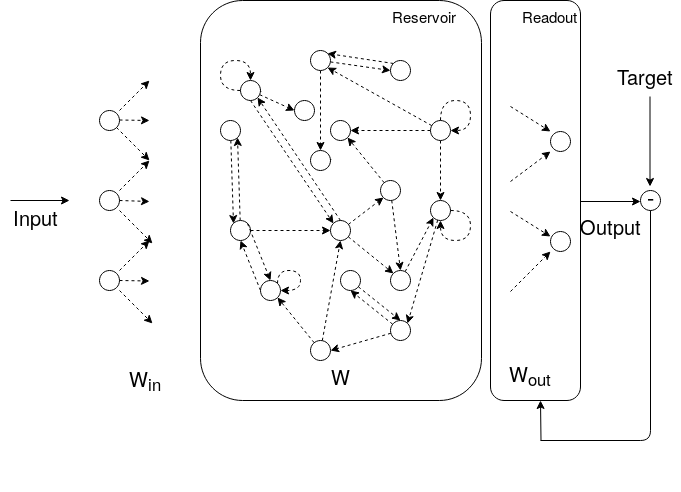
\includegraphics[width=0.7\linewidth]{immagini/RC.png}
	\caption{Reservoir Computing e allenamento del readout.}
	\label{fig:RC}
\end{figure}

Ciò significa che $\mathbf{\mathbf{W_{in}}}$ e $\mathbf{\mathbf{W}}$ sono fisse e $\mathbf{\mathbf{W_{out}}}$ varia in base all'allenamento. Tuttavia non tutte le scelte di $\mathbf{\mathbf{W_{in}}}$ e $\mathbf{\mathbf{W}}$ producono una ESN valida, il \textit{reservoir} deve essere un eco ("echo") della storia dell'input, cioè le dinamiche del \textit{reservoir} devono dipendere asintoticamente solo dai segnali di input.


\section{Le funzioni di attivazione}
Le funzioni di attivazioni alle quali si fa riferimento nella formula \ref{attivazioneesn} possono essere diverse, tra queste:
\begin{itemize}
	\item la funzione identità : $f_{id}(x)=x$ (\ref{att:(a)})
	\item la funzione logistica : $f_{logistic}(x)=  {1 \over 1+ e^{-x} }$ (\ref{att:(b)})
	\item la tangente iperbolica : $f_{tanh}(x)=  {e^{x}- e^{-x} \over e^{x}+ e^{-x} }$ (\ref{att:(c)})
\end{itemize}

\begin{figure}[h!]
	\centering
	\begin{subfigure}[b]{0.30\textwidth}
		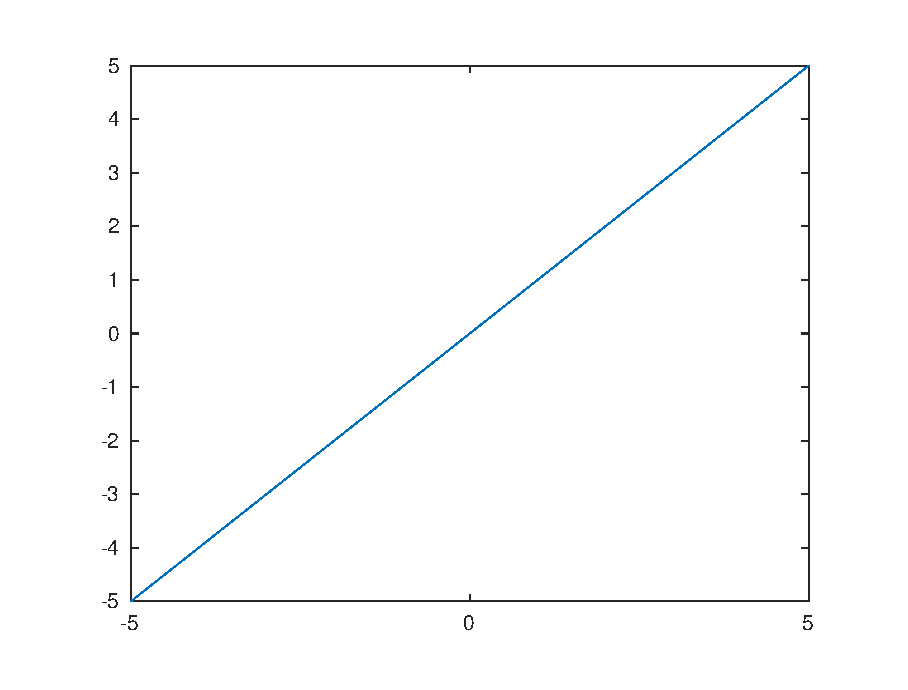
\includegraphics[width=\linewidth]{immagini/id}
		\caption{Funzione identità}
		\label{att:(a)}
	\end{subfigure}%
	\begin{subfigure}[b]{0.30\textwidth}
		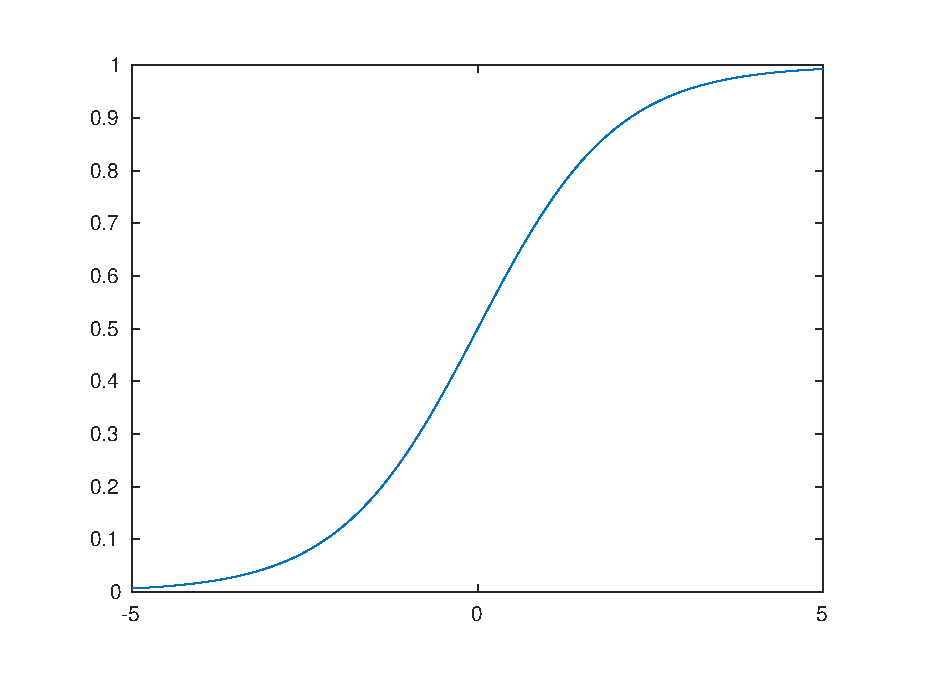
\includegraphics[width=\linewidth]{immagini/logistic}
		\caption{Funzione logistica}
		\label{att:(b)}
	\end{subfigure}%
	\begin{subfigure}[b]{0.30\textwidth}
		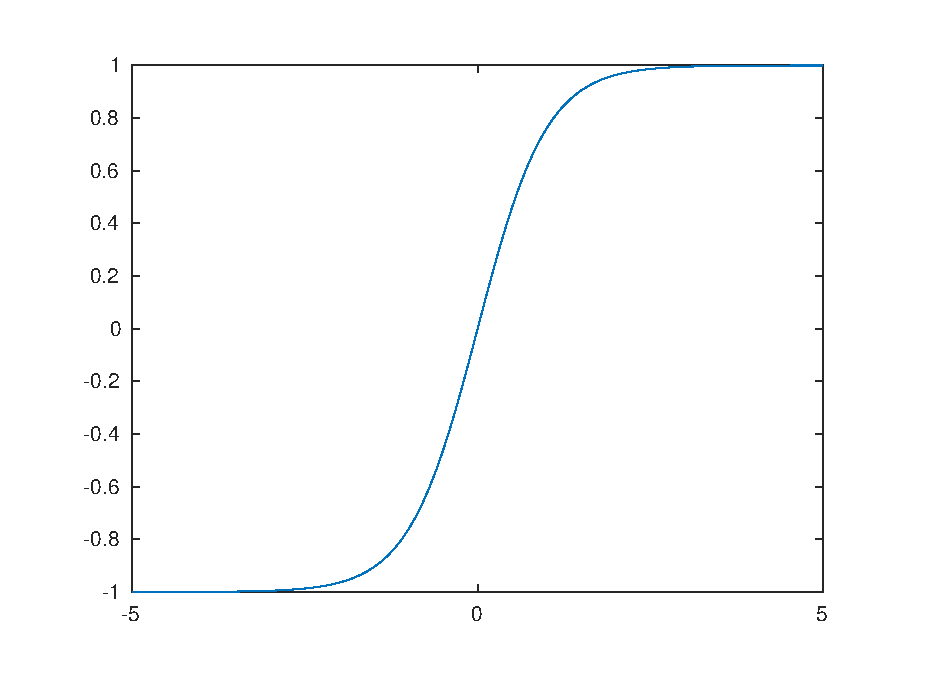
\includegraphics[width=\linewidth]{immagini/tanh}
		\caption{Tangente iperbolica}
		\label{att:(c)}
	\end{subfigure}%
	\caption{Funzioni di attivazione comuni.}\label{fattivazioni}
\end{figure}

La funzione logistica e la tangente iperbolica sono le più usate, l'idea è che si può mappare ogni numero reale in un numero nell'intervallo $[0,1]$ e rispettivamente in $[-1,1]$, in questo modo si può dimostrare che una combinazione di queste funzioni può approssimare ogni funzione non lineare.\\

\section{Leaking integration}
Le unità nelle reti  sigmoidali standard non hanno memoria; il loro valore ad un tempo $n+1$ dipende solo parzialmente ed indirettamente dai valori precedenti. Perciò queste reti si adattano al meglio per sistemi discreti nel tempo, d'altra parte è difficile l'apprendimento di dinamiche lente come onde sinusoidali molto lente. Per apprendere sistemi lenti e variabili in uno spazio continuo è più adeguato utilizzare delle reti con dinamiche continue. Per questo già in 
\cite{h} viene introdotto un approccio ibrido che usa reti discrete nel tempo che approssimano delle reti continue grazie alle unità con \textit{leaky integration}.
In questo caso una semplificazione dell'equazione per il calcolo dello stato delle unità è la seguente:

\begin{equation} \label{attivazionelr}
\mathbf{x}(\mathit{t})=(1-\alpha) \mathbf{x}(\mathit{t - 1} ) + \alpha \mathit{f}_\mathit{x} (\mathbf{u}(\mathit{t}), \mathbf{x}(\mathit{t} - 1)) = 
\end{equation}
\begin{displaymath}
(1-\alpha) \mathbf{x}(\mathit{t - 1} ) + \alpha f(\mathbf{W_{in}}u(\mathit{t}) + \mathbf{Wx}(\mathit{t - 1} ) + \mathbf{b} )
\end{displaymath}  

dove $\alpha \in (0,1]$ è il \textit{leaking decay rate}, se si  
imposta $\alpha=1$ si ottiene una ESN standard.

\section{Echo State Property}
Una ESN valida soddisfa la cosiddetta \textit{Echo State Property} (ESP) (Jager,2001). Questa dice che lo stato in cui la rete si trova dopo l'analisi di una lunga sequenza di input dipende solo dalla sequenza stessa. La dipendenza dallo stato iniziale della rete è progressivamente persa quando la lunghezza della sequenza di input tende all'infinito. Analogamente, lo stato corrente della rete $\mathbf{x}(\mathit{t})$ è una funzione della storia dell'input indipendentemente dai valori iniziali dello stato. In formule la ESP può essere espressa come segue:
\begin{displaymath}
\forall s_n(\mathbf{u}) = [\mathbf{u}(1),...,\mathbf{u}(\mathit{n})] \in (\mathbb{R}^{N_u})^n sequenza\ di\ input\ di\ lunghezza\ n,
\end{displaymath}
\begin{equation}\label{ESP}
\forall \mathbf{x}, \mathbf{x'} \in \mathbb{R}^{N_r}:
\end{equation}
\begin{displaymath}
 \Vert \mathit{f_x}(s_n(\mathbf{u}), \mathbf{x}) - \mathit{f_x}(s_n(\mathbf{u}), \mathbf{x'}) \Vert \rightarrow 0\ per\ \mathit{n} \rightarrow \infty
\end{displaymath}
che significa che la differenza tra gli stati che la rete assume dopo che viene valutata una sequenza di input di lunghezza $n$ tende a zero al tendere di $n$ ad infinito, per ogni scelta iniziale dello stato.\\
Jaeger ha fornito due condizioni, rispettivamente necessaria e sufficiente, affinchè una ESN goda di questa proprietà. La condizione necessaria è che il raggio spettrale, ovvero il maggiore degli autovalori in modulo, della matrice dei pesi del \textit{reservoir} sia minore di uno.
\begin{equation}\label{raggiospettrale}
\rho(\mathbf{W})<1
\end{equation}
Se questa condizione viene violata, il reservoir è localmente asintoticamente instabile nello stato $\mathbf{0} \in \mathbb{R}^{N_r}$ e la echo state property non può essere garantita se la sequenza nulla è un input ammissibile per il sistema.\\
La condizione sufficiente per la validità della proprietà è che il massimo valore singolare di \textbf{W} sia minore di uno:
\begin{equation}\label{raggiospettrale2}
\sigma(\mathbf{W}) <1
\end{equation}
Ciò assicura la stabilità globale del sistema e la presenza di "stati echo", garantendo così la echo state property.\\
Una caratteristica molto importante evidenziata in \cite{Markovianfactor:paper}  è la contrattività delle dinamiche dello stato.\\
La contratività della funzione di transizione dello stato $\mathit{f_x}$ è una condizione sufficiente ma non necessaria per garantire la ESP.
